\subsection{Requirements}
\label{subsec:Requirements}
Depending on the features you wish to access and the platform you prefer using, you should head to the corresponding website of each requisite. For each method, the requirements and their details are explained in the following segments. 

\subsubsection{Python}
This requirement can be skipped if you plan on relying solely on the Docker platform to start ABAI.\\

First, please head over to the official \href{https://www.python.org/}{Python website} and navigate to the download page. Once you see the versions of python available to download, select the latest released stable version and follow the instructions to download and install python on your machine. 

\subsubsection{Docker}
This requirement can be skipped if you plan on relying solely on the command line terminal and Python to start ABAI. \\

First, please head over to the official \href{https://www.docker.com/}{Docker website} and navigate to their Docker Desktop download page under the products section. Alternatively (or if your OS environment doesn't have a desktop deployable version), you can try to follow the official Docker Engine \href{https://docs.docker.com/engine/install/}{installation guide}.
\clearpage

\subsection{Download}
\label{subsec:Download}
Now that you meet the requirements from the previous steps, you are ready to download the tool. For this, download the compressed ABAI .ZIP project folder directly from it's \href{https://github.com/UNamurCSFaculty/2324_INFOB318_ABAI2}{GitHub repository} \href{https://github.com/UNamurCSFaculty/2324_INFOB318_ABAI2/releases/tag/ABAI-0.0.1}{release page}.
\begin{center}
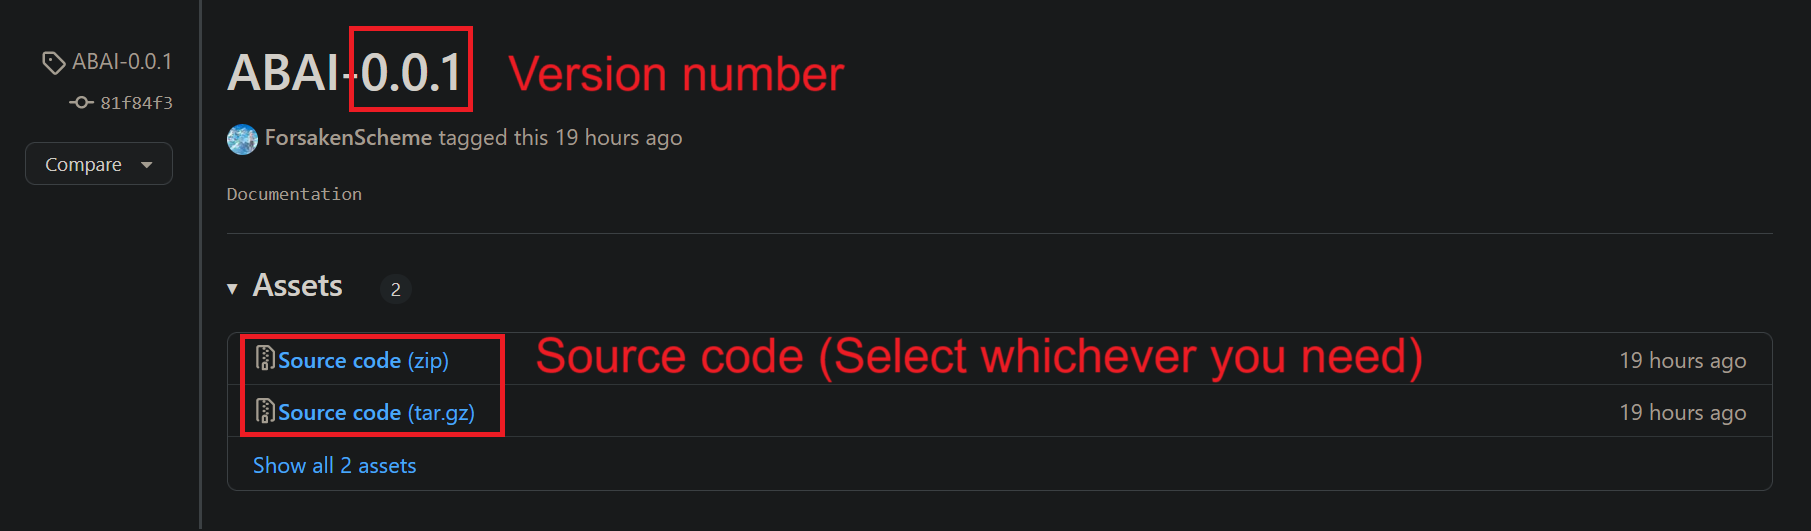
\includegraphics[width=17cm]{Images/Download/releases.png}
\end{center}
\subsection{Extract}
\label{subsec:Extract}
Once the download is complete, select your favourite extraction method (built-in OS feature or any additional file archiver software like \href{https://7-zip.org/}{7-Zip}), and extract the content of the compressed project folder into the installation folder at the location of your choice.
\begin{center}
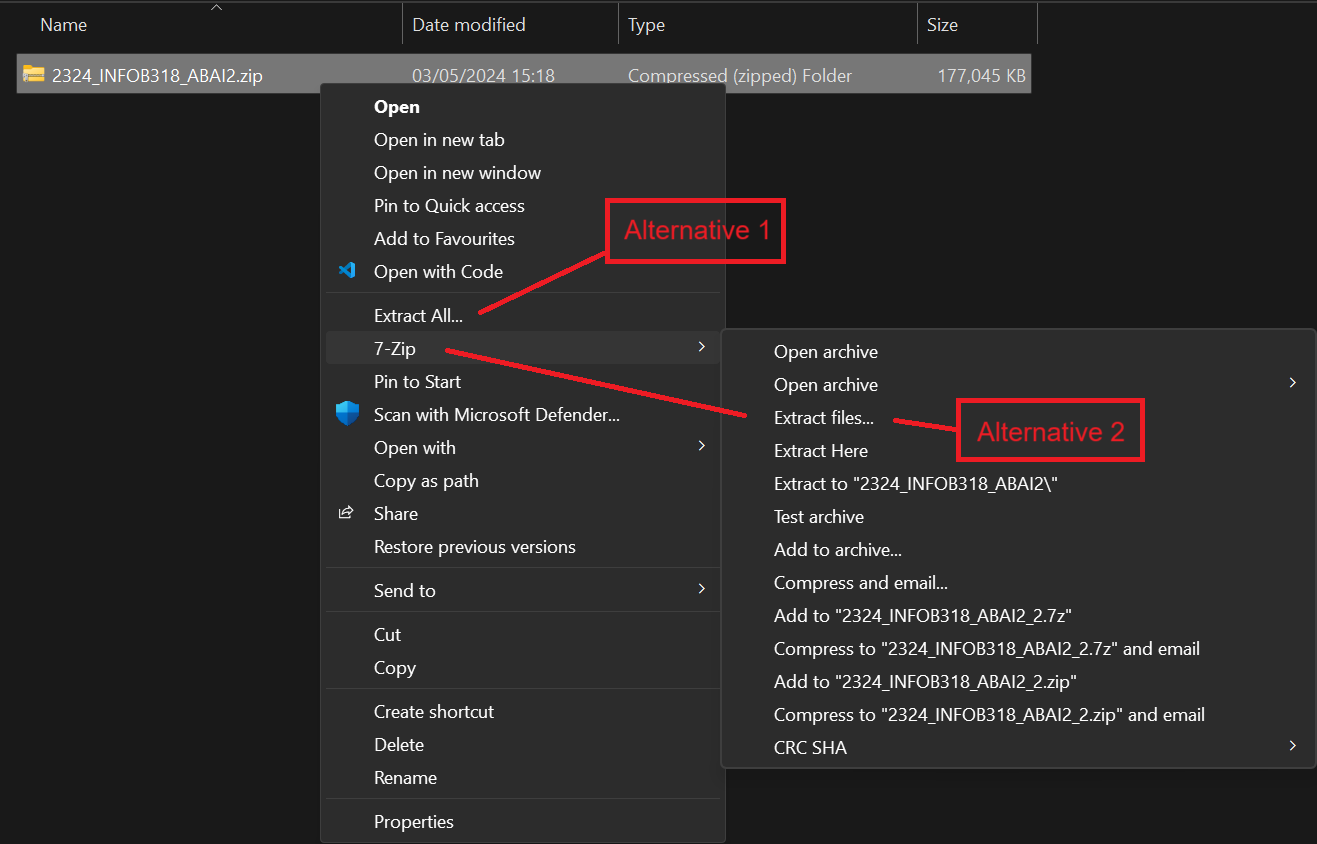
\includegraphics[width=17cm]{Images/Extract/Extraction.png}
\end{center}

After extraction, you should have the following folders: 
\begin{center}
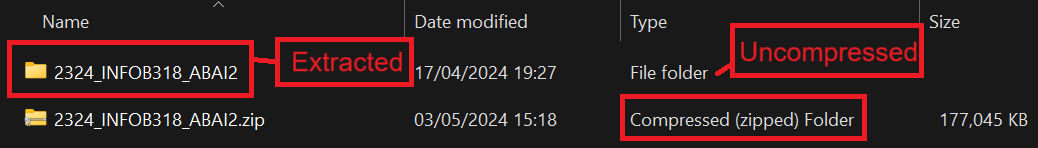
\includegraphics[width=17cm]{Images/Extract/after_extraction.png}
\end{center}

The uncompressed folder should contain the file structure shown as preview on the GitHub project page. The compressed folder can be safely deleted after having extracted and placed the \texttt{2324\_INFOB318\_ABAI2-[\texttt{version number}]} folder where you want to store it to run the program from.


\subsection{First steps}
\label{subsec:First steps}
After finishing the previous steps (\hyperref[subsec:Requirements]{2.1}, \hyperref[subsec:Download]{2.2}, \hyperref[subsec:Extract]{2.3} and \hyperref[subsec:First steps]{2.4}), you should now be able to start the tool. The steps to start ABAI may vary depending on what features and platform you plan to use. A walk-trough with steps for the local and web based application can be found at section \hyperref[subsubsec:Local application]{2.4.1 Local application} and \hyperref[subsubsec:Web application]{2.4.2 Web application}.

\subsubsection{Local application}
\label{subsubsec:Local application}
If you want to start the local application, you will have to use the standalone \textbf{python} GUI. For this, proceed as follows : 

\begin{itemize}
  \item Navigate to the \texttt{2324\_INFOB318\_ABAI2-[\texttt{version number}]} folder and, inside the folder, run the command:\begin{codebox}
    \texttt{pip install -r requirements.txt}.
  \end{codebox}
  \item Still inside the folder, run the command: 
  \begin{codebox}
    \texttt{python -O .\textbackslash code\textbackslash backend\textbackslash main.py}.
  \end{codebox}
  \item A window will open, this is the python GUI menu. 
\end{itemize}
\clearpage
\subsubsection{Web application}
\label{subsubsec:Web application}
If you want to start the web application, you are able to use the command-line terminal with Python or Docker (Docker Desktop GUI). 

\paragraph{\fontsize{14}{17}\selectfont Python}
\begin{itemize}
  \item First, open a terminal and navigate to the \texttt{2324\_INFOB318\_ABAI2-[\texttt{version number}]} folder.
  \item Inside the folder, run the command: 
  \begin{codebox}
    \large\texttt{pip install -r requirements.txt}.
  \end{codebox}
  \item Still inside the folder, run the command:
  \begin{codebox}
    \large\texttt{python -O .\textbackslash code\textbackslash django\_abai\textbackslash manage.py runserver 0.0.0.0:8000}.
  \end{codebox}
  \item Open your favorite browser and go to: \url{http://localhost:8000/}.
\end{itemize}
\paragraph{\fontsize{14}{17}\selectfont Docker}
\begin{itemize}
  \item First, open a terminal and navigate to the \texttt{2324\_INFOB318\_ABAI2-[\texttt{version number}]} folder.
  \item From the current working directory, run the command:
  \begin{codebox}
    \texttt{docker-compose -f docker/docker-compose.yml build}.
  \end{codebox}
  \item Then,  still from the \texttt{2324\_INFOB318\_ABAI2-[\texttt{version number}]} current working directory, run the command:
  \begin{codebox}
    \texttt{docker-compose -f docker/docker-compose.yml up abai-website}
  \end{codebox}
  \textbf{or} \\
  On the Docker Desktop GUI chose the abai-web image and start the container with a name of your choice and specify the port 8000.
  \item Open your favourite browser and go to: \\
  \url{http://172.28.112.1:8000/} (accessible from any device in the local network) \\
  \textbf{or} \\
  \url{http://localhost:8000/} (accessible from local host device only).
\end{itemize}


